\documentclass[12pt]{article}
\usepackage[utf8]{inputenc}
\usepackage{graphicx}
\usepackage[spanish,es-tabla]{babel}
\usepackage{amsmath}
\usepackage[a4paper,margin=1in]{geometry}
\usepackage{subcaption}
\usepackage{amssymb}
\usepackage[hidelinks]{hyperref}
\usepackage{mathtools}
\usepackage[table,xcdraw]{xcolor}
\usepackage[style=ieee, backend=biber]{biblatex}
\usepackage{enumitem}
\usepackage{array}
\usepackage{longtable}
\usepackage{csquotes}
\usepackage{circuitikz}
\graphicspath{{Figuras/}}           
\usepackage{float}
\usepackage{setspace}
\onehalfspacing

\addbibresource{bibliografía.bib}   
\hypersetup{
    colorlinks=true,
    linkcolor=blue,    
    citecolor=blue,
    urlcolor=blue,
    filecolor=blue
}

\begin{document}       
\renewcommand{\figureautorefname}{Fig.}
\renewcommand{\tableautorefname}{Tab.}
\renewcommand{\equationautorefname}{Ec.}

\begin{titlepage}
\thispagestyle{empty}
\begin{tikzpicture}[remember picture,overlay]
    \node[opacity=0.2,anchor=center] at (current page.center) 
        {
\includegraphics[width=0.9\paperwidth]{decoracion_a.png}};
\end{tikzpicture}
\begin{center}
    
\includegraphics[width=15cm]{unc_fcefyn_logo.png} \\ [0.5cm]
    \LARGE Universidad Nacional de Córdoba \\ [0.5cm] 
    \large Facultad de Ciencias Exactas, Físicas y Naturales \\ 
    \vspace{40pt}
    \large Sistemas de Radiocomunicación \\ [0.2cm]
    \large Trabajo Práctico N°1 \\
    \vspace{60pt}
    \LARGE Regulación de las Telecomunicaciones y Espectro \\
    \vspace{60pt}
    \begin{table}[!h]
        \centering
        \begin{tabular}{ll}
            \multicolumn{1}{c}{Nombre} & \multicolumn{1}{c}{DNI} \\
            Mendes Rosa, Agustín             & 44.517.201 \\
            Monja, Ernesto Joaquín           & 43.873.728
        \end{tabular}
    \end{table}
    \vspace{20pt}
    \begin{table}[!h]
        \centering
        \begin{tabular}{ll}
            \multicolumn{1}{c}{Docentes} & Esp. Ing. Liendo, Carlos Guillermo \\
                                         & Ing. Dadam, Federico Tomás \\
        \end{tabular}
    \end{table}
    \vfill
        {\small Córdoba, República Argentina\\
                Año 2026}
\end{center}
\end{titlepage}
\newpage

\tableofcontents
\newpage



\section{Introducción}
\label{sec_1}
En el presente informe se desarrolla un análisis integral sobre la regulación de las telecomunicaciones y la gestión del espectro radioeléctrico, elementos fundamentales para el ordenamiento y desarrollo de los \textit{Sistemas de Radiocomunicaciones}. Para ello, se aborda el rol de los principales organismos reguladores, comenzando por la Unión Internacional de Telecomunicaciones (\textit{UIT}) a nivel global y su impacto mediante el Reglamento de Radiocomunicaciones, hasta llegar a la esfera nacional con la intervención del Ente Nacional de Comunicaciones (\textit{ENACOM}) y el marco normativo vigente, como la Ley 27.078.

Adicionalmente, el documento presenta una aplicación práctica de estos conceptos mediante el uso de la plataforma interactiva \textit{HERTZ} y el estudio de referencias técnicas sobre propagación electromagnética. A través de este análisis, se identifican las bandas de frecuencia, resoluciones y características operativas para diversas tecnologías actuales, tales como redes \textit{Wi-Fi}, telefonía móvil $4G$, sistemas satelitales y protocolos para Internet de las Cosas (\textit{IoT}), contemplando también las políticas de espectro, el dividendo digital y los estándares de salud pública frente a las radiaciones no ionizantes.



\section{Desarrollo}
\label{sec_2}
\subsection{UIT y Normativa Internacional}
\label{sec_2.1}
\subsubsection{Origen, estructura y funcionamiento de la \textit{UIT}}
\label{sec_2.1.1}
La \textit{UIT} (Unión Internacional de Telecomunicaciones) es el organismo especializado de las Naciones Unidas, orientado a diversos aspectos de las Tecnologías de la Información y la Comunicación (\textit{TIC}). Su origen se remonta a $1865$ en París, cuando se celebró el primer acuerdo telegráfico y nació la Unión Telegráfica Internacional (\textit{UTI}). Posteriormente, en $1932$, se adoptó el nombre de Unión Internacional de Telecomunicaciones. \cite[p. 4]{b1}

La \textit{UIT} organiza sus actividades mediante conferencias y reuniones divididas en tres ``Sectores'':
\begin{itemize}
    \item \underline{Sector de Radiocomunicaciones (\textit{UIT-R})}: Determina las características técnicas y los procedimientos operativos de servicios inalámbricos.
    \item \underline{Sector de Normalización de las Telecomunicaciones (\textit{UIT-T})}: Contribuye a difundir el acceso equitativo, sostenible y con un costo razonable a las Tecnologías de la Información y la Comunicación.
    \item \underline{Sector de Desarrollo de las Telecomunicaciones (\textit{UIT-D})}: Facilita y mejora el desarrollo de las telecomunicaciones mediante actividades de asesoramiento en materia de política, reglamentación, financiación de las telecomunicaciones, opciones tecnológicas de bajo costo y asistencia técnica directa en la gestión de recursos humanos y la elaboración de iniciativas encaminadas al desarrollo rural y al acceso universal.
\end{itemize}

Entre sus objetivos principales se destacan:
\begin{itemize}
    \item Formula normas mundiales destinadas a los fabricantes, operadores, proveedores de servicios, usuarios y entidades interesadas.
    \item Facilita la reglamentación y coordinación de asuntos relacionados con el espectro radioeléctrico, con vistas a mejorar la eficiencia en su uso.
    \item Administra las órbitas satelitales.
    \item Contribuye a la promoción y coordinación de la asistencia técnica y la expansión de las telecomunicaciones en los países en desarrollo.
    \item Edita el Reglamento de las Radiocomunicaciones (RR) con vigencia para todos los países miembros. \cite[p. 4-5]{b1}
\end{itemize}



\subsubsection{Análisis de Estándar: Coordinación de satélites geoestacionarios}
\label{sec_2.1.2}
El estándar de Coordinación de satélites geoestacionarios es administrado por el \textit{UIT-R}. Dado que la Órbita de Satélites Geoestacionarios (\textit{OSG}) y el espectro radioeléctrico son recursos naturales limitados, el \textit{UIT-R} garantiza su acceso equitativo y libre de interferencias mediante el Reglamento de Radiocomunicaciones (\textit{RR}), específicamente bajo los procedimientos de sus Artículos $9$ y $11$.

Para estandarizar y agilizar este proceso multilateral de coordinación entre países antes del lanzamiento de un satélite, el \textit{UIT-R} define metodologías técnicas clave (principalmente en su Serie \textit{S} de Recomendaciones):
\begin{itemize}
    \item \underline{Arco de Coordinación:} Define umbrales angulares para identificar rápidamente redes que requieren coordinación obligatoria por cercanía. La \autoref{fig:fig_1} muestra algunos de los grados para arcos de acuerdo a las bandas.
    \begin{figure}[H]
        \centering
        \fbox{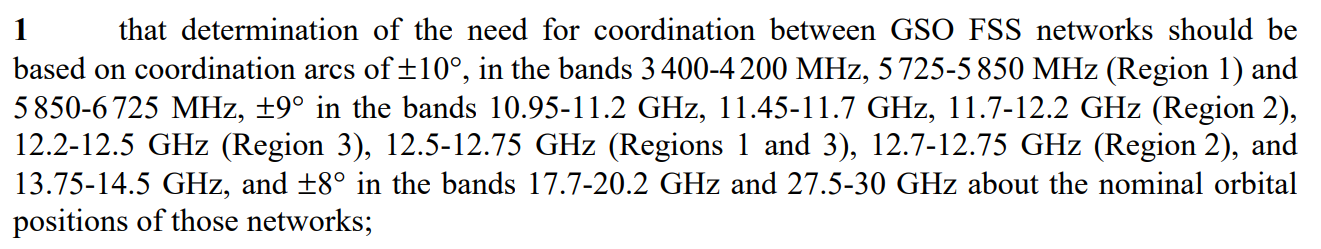
\includegraphics[width=0.8\linewidth]{Figura 1.png}}
        \caption{Arcos de Coordinación para distintas bandas. \cite{b2}}
        \label{fig:fig_1}
    \end{figure}
    
    \item \underline{Criterio de temperatura de ruido ($\Delta T/T$):} Permite eximir el proceso de coordinación si una administración demuestra analíticamente que las emisiones de su satélite no incrementarán la temperatura de ruido equivalente de una red preexistente en más de un $6 \, [\%]$.
\end{itemize}

La aplicación estricta de estos estándares resulta vital para la sostenibilidad espacial. Su cumplimiento evita el solapamiento destructivo de señales y previene el colapso de los servicios satelitales de telecomunicaciones a nivel global. \cite{b2}



\subsubsection{Impacto global de la \textit{UIT}}
\label{sec_2.1.3}
La \textit{UIT} está conformada por $193$ naciones o estados miembros, agrupados en $3$ regiones que corresponden a distintas zonas geográficas, donde Argentina pertenece a la Región $2$ tal como muestra la \autoref{fig:fig_2}.
\begin{figure}[H]
    \centering
    \fbox{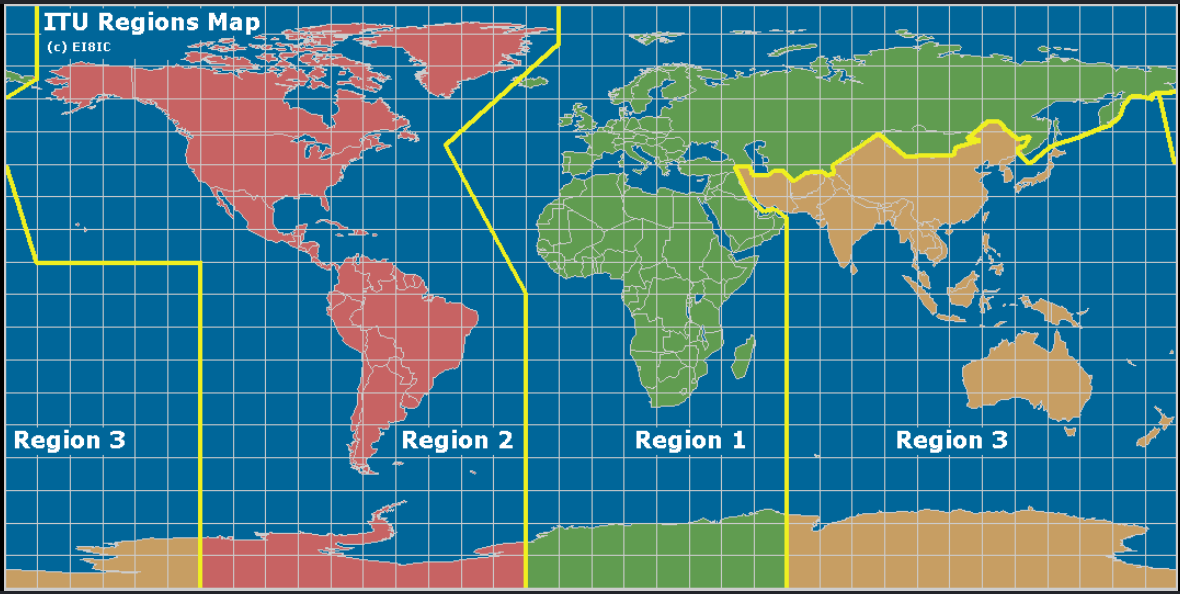
\includegraphics[width=0.9\linewidth]{Figura 2.png}}
    \caption{Mapa de Regiones \textit{UIT}. \cite{b3}}
    \label{fig:fig_2}
\end{figure}

Esta división se realizó con el fin de planificar, atribuir y asignar las bandas de frecuencias del espectro radioeléctrico, de manera tal que todos los países puedan compartir este recurso natural no renovable en forma equitativa y armonizada. \cite[p. 4-5]{b1}

Además, cuenta con más de $700$ miembros de organizaciones no gubernamentales, entre ellos las Universidades. Entre los actores relevantes del sector privado y académico se destacan corporaciones tecnológicas y operadores globales (como Ericsson, Huawei, Nokia, Microsoft, Telefónica e Intelsat), organismos de la industria de las telecomunicaciones (como la GSMA o el IEEE), y diversas casas de estudios superiores y centros de investigación a nivel mundial, incluyendo representaciones de universidades argentinas que colaboran en el desarrollo de nuevos estándares tecnológicos. \cite{b4}

\subsubsection{Reglamento de Radiocomunicaciones}
\label{sec_2.1.4}
El Reglamento de Radiocomunicaciones (\textit{RR}) es el tratado internacional por el cual se rige el uso del espectro de radiofrecuencias y de las órbitas de satélites geoestacionarios y no geoestacionarios. Contiene la totalidad de reglas a las que deben someterse las radiocomunicaciones en los países miembros, además de las correcciones de las anteriores ediciones y los nuevos reglamentos surgidos por el avance tecnológico de los últimos años. Su contenido se divide en $4$ volúmenes y una Serie separada:
\begin{itemize}
    \item Volumen $1$ – Artículos
    \item Volumen $2$ – Apéndices
    \item Volumen $3$ – Resoluciones y Recomendaciones
    \item Volumen $4$ – Recomendaciones \textit{UIT-R} incorporadas por referencia
    \item Serie separada – Mapas que deben ser utilizados en el Apéndice 27 (Rev.CMR-12)
\end{itemize}

La UIT organiza cada tres o cuatro años la Conferencia Mundial de Radiocomunicaciones (CMR), una reunión donde se definen los futuros cambios que se implementarán en los temas que le competen, para luego editar el \textit{RR} (el último documento disponible es el de la reunión en $2023$). El Reglamento define los siguientes aspectos:
\begin{itemize}
    \item La asignación de diferentes bandas de frecuencia a diferentes servicios de radio, dividida en bloques cuyo tamaño varía según las necesidades de cada servicio.

    \item Los parámetros técnicos obligatorios que deben observarse por parte de las estaciones de radio, especialmente las emisoras.

    \item Los procedimientos para garantizar la compatibilidad técnica, registro formal y protección en el Registro Internacional de Frecuencias de las asignaciones de frecuencia a las estaciones de radio de los gobiernos nacionales.

    \item Otros procedimientos y disposiciones operativas.
\end{itemize}

Sólo la Conferencia Mundial de Radiocomunicaciones (\textit{CMR}) puede introducir cambios en el Cuadro de Atribución de Frecuencias y en el propio Reglamento.



\subsection{\textit{ENACOM} y Regulación Nacional}
\label{sec_2.2}
\subsubsection{Origen y funciones del \textit{ENACOM}}
\label{sec_2.2.1}
El Ente Nacional de Comunicaciones (\textit{ENACOM}) es el ente de regulación de Argentina que establece el marco legal sobre las comunicaciones, en base a los acuerdos logrados por la \textit{UIT} bajo el consenso de los países de cada región. 

Es el encargado de atribuir las bandas a los distintos servicios mediante reglamentaciones, decretos y leyes, de adjudicar las frecuencias y canales al plan de comunicaciones nacional, asignar el uso de las distintas frecuencias y canales establecidos en el plan a los distintos licenciatarios, y controlar el cumplimiento de sus obligaciones en el uso del espectro asignado.

El \textit{ENACOM} fue creado en diciembre de $2015$ mediante el Decreto $267/15$. Surgió de la unificación de los organismos \textit{AFSCA} (Autoridad Federal de Servicios de Comunicación Audiovisual, encargado de los medios de comunicación aplicando la Ley de Medios N.º 26.522) y \textit{AFTIC} (Autoridad Federal de Tecnologías de Información y Comunicaciones, encargado de telecomunicaciones que no refieran a medios de radiocomunicación).

Dentro de las principales funciones del ente se encuentran:
\begin{itemize}
    \item Implementar un marco normativo homogéneo adecuado para el desarrollo de la industria, que redunde en el beneficio de usuarios y consumidores con el objeto de que puedan acceder a una mayor cantidad y diversidad de servicios a menores precios.

    \item Facilitar la defensa de la competencia contra toda forma de distorsión de los mercados, beneficiando a los consumidores y evitando las distorsiones en la competencia, como la ejecución selectiva de sanciones, el otorgamiento discrecional de licencias y cualquier mecanismo de premios y castigos arbitrarios u otras prácticas distorsivas.

    \item Resguardar el bienestar general y las condiciones de igualdad en el acceso de la población a servicios de calidad contribuyendo a eliminar la brecha digital.

    \item Mantener una política pública de acción rápida y eficaz que establezca un sendero racional en el desarrollo del sector, adaptando la regulación a los requerimientos del sector y la sociedad y colaborando en el re-ordenamiento del mercado de las comunicaciones.

    \item Garantizar la más amplia libertad de prensa, el pluralismo y el acceso a la información, fomentar el desarrollo de las nuevas tecnologías de la información y las comunicaciones, y avanzar hacia la convergencia entre las distintas tecnologías disponibles, garantizando la seguridad jurídica para fomentar las inversiones en infraestructuras.

    \item Mantener y garantizar el adecuado funcionamiento de los distintos actores del sector de las comunicaciones, adaptando de manera periódica las reglas de concentración por impacto de las tecnologías y la aparición de nuevos factores o situaciones.
\end{itemize}



\subsubsection{Identificación de Bandas y Servicios}
\label{sec_2.2.2}
Para la identificación y gestión del espectro radioeléctrico a nivel nacional, el \textit{ENACOM} dispone de la plataforma pública e interactiva \textit{HERTZ}. Este sistema web funciona como la interfaz gráfica del Cuadro Nacional de Atribución de Bandas de Frecuencias (\textit{CNAF}), permitiendo a los usuarios consultar rangos de frecuencias o servicios específicos para conocer rápidamente su atribución (jerarquía primaria o secundaria), denominación técnica y el marco normativo o resoluciones vigentes.

El uso de esta herramienta resulta indispensable para la consulta regulatoria y la planificación libre de interferencias. La aplicación práctica de este portal, mediante el relevamiento de los parámetros legales y técnicos para diversas tecnologías actuales, se desarrolla en detalle en la \autoref{sec_2.5} del presente informe.


\subsection{Espectro y Políticas Públicas}
\label{sec_2.3}
\subsubsection{Dividendo Digital}
\label{sec_2.3.1}
Se conoce como ``Dividendo Digital'' a la porción del espectro radioeléctrico que queda liberada tras migrar de la televisión analógica a la televisión digital.

La Televisión Digital Terrestre (\textit{TDT}) tiene la capacidad de transmitir los datos de forma más compacta, es decir, en el mismo ancho de banda que antes ocupaba un canal de televisión analógica, hoy pueden transmitirse múltiples canales digitales. De esta manera, una gran porción del espectro radioeléctrico queda vacío (en la banda de \textit{UHF}).

Por recomendación de la \textit{UIT}, los países destinan este dividendo digital a los servicios de telefonía móvil para internet de banda ancha (\textit{4G/LTE} y \textit{5G}).

A nivel nacional la Resolución $008/15$ dejó sin efecto las atribuciones en la banda de $470$ a $512 \, [MHz]$ (canales $14$ a $20$ de \textit{UHF}) de Servicio Fijo y Móvil Terrestre para destinarla a servicios de televisión digital tal como muestra la \autoref{fig:fig_3}
\begin{figure}[H]
    \centering
    \fbox{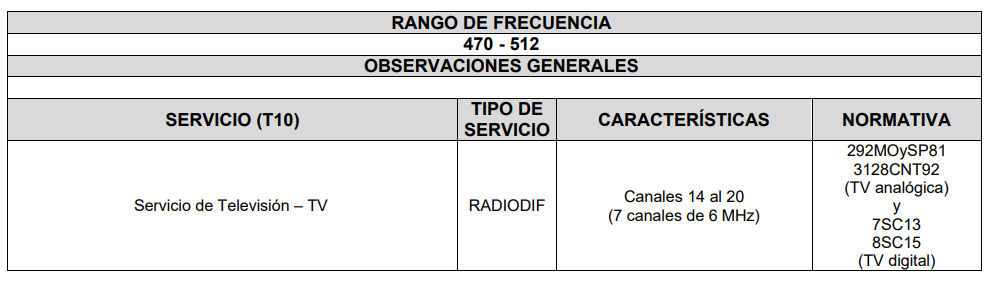
\includegraphics[width=0.9\linewidth]{Figura 3.png}}
    \caption{Banda de $470-512 \, [MHz]$. \cite{b5}}
    \label{fig:fig_3}
\end{figure}

A nivel regional, la gestión del ''Dividendo Digital'' ha buscado la armonización del espectro, adoptando mayoritariamente la banda de $700 \, [MHz]$ (conocida como canalización \textit{APT700}) para el despliegue de servicios móviles de cuarta generación. A continuación, se detallan $2$ ejemplos sudamericanos:
\begin{itemize}
    \item \underline{Ecuador:} El organismo regulador, la Agencia de Regulación y Control de las Telecomunicaciones (\textit{ARCOTEL}), dispuso la liberación de la banda de $700 \, [MHz]$ (específicamente el segmento comprendido entre $698$ y $806 \, [MHz]$) tras el apagón analógico. Este espectro fue atribuido al Servicio Móvil Avanzado (\textit{SMA}) para expandir la cobertura de \textit{4G LTE}, especialmente en zonas rurales debido a la excelente propagación de estas frecuencias. \cite{b5.1}
    
    \item \underline{Uruguay:} La Unidad Reguladora de Servicios de Comunicaciones (\textit{URSEC}) siguió una política similar, atribuyendo la banda del dividendo digital ($700 \, [MHz]$) al servicio móvil. Mediante subastas públicas, asignó estos bloques a los operadores de telecomunicaciones (como Antel, Claro y Movistar) con exigencias estrictas de cobertura en rutas nacionales y poblaciones del interior del país, aprovechando las características de la banda para cerrar la brecha digital. \cite{b5.2}
\end{itemize}



\subsubsection{Servicio Universal}
\label{sec_2.3.2}
Se define como un conjunto de servicios de \textit{TICs} que el Estado debe garantizar a toda la población con determinada calidad y precios accesibles, sin importar la geografía o la condición socioeconómica.

Se sostiene mediante un fideicomiso (o fondo fiduciario) al que aportan los licenciatarios de servicios de telecomunicaciones en una cantidad equivalente al $1\%$ de los ingresos totales devengados por la prestación de los servicios de \textit{TIC}. Los fondos del Servicio Universal se aplican por medio de programas específicos, definidos por \textit{ENACOM}. \cite{b6}

Se aprobó un nuevo régimen en septiembre de 2025, el Reglamento General del Servicio Universal, derogando el marco regulatorio vigente desde 2020. Las modificaciones que destacan se enumeran a continuación:

\begingroup
\footnotesize
\begin{longtable}
    {|>{\centering\arraybackslash}m{3.2cm}
     |>{\centering\arraybackslash}m{5.6cm}
     |>{\centering\arraybackslash}m{5.6cm}|} \hline
     & \textbf{Reglamento General 2020} & \textbf{Reglamento General 2025} \\ \hline
    \endfirsthead
    
    \multicolumn{3}{c}{\textit{Continuación de la página anterior}} \\ \hline
    \textbf{Eje / Aspecto} & \textbf{Reglamento General 2020} & \textbf{Reglamento General 2025} \\ \hline
    \endhead
    
    \hline 
    \multicolumn{3}{c}{\textit{Continúa en la página siguiente...}} \\
    \endfoot
    
    \hline
    \caption{Comparativa del Reglamento General del Servicio Universal (2020 vs. 2025).}
    \label{tab:servicio_universal_2020_2025} \\
    \endlastfoot

    \textbf{Norma de Aprobación} & 
        Res. \textit{ENACOM} N.º 721/2020. & 
        Res. \textit{ENACOM} N.º 1182/2025. \\ \hline
        
    \textbf{Administración del Fondo} & 
        \textbf{Esquema Fiduciario:} El fondo se administra mediante la figura de un Fondo Fiduciario privado/bancario según el Art. 21 de la Ley 27.078. & 
        \textbf{Administración Directa ENACOM:} Administración directa de la Autoridad de Aplicación (\textit{ENACOM}) para reducir costos operativos. \\ \hline
        
    \textbf{Aporte de Inversión} & 
        1\% de los ingresos totales devengados por la prestación de Servicios TIC. & 
        Sin modificación. \\ \hline
        
    \textbf{Deducciones e Interconexión} & 
        Se permitían deducciones de costos de interconexión sin exigencia de trazabilidad fiscal detallada del prestador interconectado. & 
        Para deducir importes por costos de interconexión, es obligatorio identificar el CUIT del prestador interconectado para evitar doble contabilización o elusión. \\ \hline
        
    \textbf{Mecanismo de Compensación por Proyectos} & 
        Cancelación parcial impositiva/aporte de hasta un $30\%$ del aporte mensual por ejecución de proyectos aprobados. & 
        \textbf{Certificado de Crédito de Aporte al Servicio Universal:} Se emite un certificado formal una vez aprobada la rendición de cuentas, aplicable al aporte mensual según fije cada programa. \\ \hline
        
    \textbf{Sistema para Declaraciones Juradas y Pagos} & 
        Presentaciones mediante plataformas administrativas previas y formularios de liquidación independientes. & 
        Unificación en el Sistema \textit{HERTZ}. Digitalización y centralización obligatoria de las Declaraciones Juradas y liquidaciones a través de la plataforma \textit{HERTZ} (Res. 926/2025). \\ \hline
        
    \textbf{Enfoque de Programas y Prioridades} & 
        Reducción de la brecha digital enfocada en conectividad social (Barrios Populares-RENABAP, instituciones públicas, zonas rurales e infraestructura de emergencia). & 
        Alineado al Plan Nacional de Infraestructura Crítica (Res. 359/2025). Prioriza redes mayoristas neutrales, banda ancha de alta velocidad, IA, Centros de Datos y reestructuración de programas previos. \\ \hline
\end{longtable}
\endgroup



\subsubsection{Operador Móvil Virtual (\textit{OMV})}    \label{sec_2.3.3}
Un Operador Móvil Virtual (\textit{OMV}) o Mobile Virtual Network Operator (\textit{MVNO}) es una empresa de telecomunicaciones que presta servicios de telefonía e internet móvil a usuarios finales bajo su propia marca, pero sin poseer espectro radioeléctrico propio ni infraestructura de red de acceso por radio (antenas, torres y radiobases). \cite{b7} \cite{b8}

El \textit{OMV} le compra al Operador Móvil con Red (\textit{OMR}, dueño de las antenas) capacidad de red al por mayor (minutos, SMS, datos) y la revende al por menor a sus clientes. Según su nivel de independencia técnica, se clasifican en:
\begin{itemize}
    \item \underline{\textit{OMV} Básico (\textit{Light MVNO}):} Solo maneja la marca, el marketing, la venta de \textit{SIMs} y la atención al cliente. Las tarjetas \textit{SIM} son emitidas por el \textit{OMR} (con el logo del \textit{OMV} impreso), y la base de datos, los sistemas de cobro y los acuerdos de Roaming son gestionados por el \textit{OMR}. Además, su nivel de dependencia del \textit{OMR} es alto.

    \item \underline{\textit{OMV} Completo (\textit{Full MVNO}):} Posee su propio núcleo de red, fabrica sus propias tarjetas \textit{SIM} con su propio código de red, gestiona su base de datos de usuarios, cobros y acuerdos de roaming (puede negociar acuerdos directos con redes de otros países). Su nivel de dependencia del \textit{OMR} es bajo, si el \textit{OMR} anfitrión presenta degradación o falla en el servicio de red, puede mudar todo su sistema a otro \textit{OMR}.
\end{itemize}

La actividad de los \textit{OMV} en el país se rige por la Resolución \textit{ENACOM} 38/2016 (Reglamento de Operadores Móviles Virtuales) \cite{b9}. 

A pesar de existir la norma, la penetración histórica de los \textit{OMV} en Argentina fue lenta porque las tres grandes telefónicas con red (Claro, Telecom/Personal y Movistar) se mostraban reacias a vender capacidad a precios mayoristas competitivos. \cite{b10} Un ejemplo es el caso de ``Tuenti'', una \textit{OMV} conocida como una marca digital low-cost, que utiliza la infraestructura de Movistar para el acceso a la red.

Los \textit{OMV} no poseen bandas de frecuencia asignadas ni licencias de espectro. Operan exactamente en las mismas bandas de frecuencia que utilice el \textit{OMR} al cual le alquilan la infraestructura. Si el operador anfitrión transmite en las bandas de $700 \, [MHz]$ (Banda $28$), \textit{AWS} (Banda $4$), $1900 \, [MHz]$ (Banda $2$) o en $3.5 \, [GHz]$ (para \textit{5G}), el \textit{OMV} prestará servicio en esas mismas frecuencias.



\subsubsection{Bandas No Licenciadas}
\label{sec_2.3.4}
Las bandas no licenciadas (o de espectro libre) son segmentos del espectro radioeléctrico reservados por las autoridades de aplicación para que cualquier persona o dispositivo pueda transmitir datos sin necesidad de abonar una licencia ni solicitar una adjudicación exclusiva de frecuencia.

A nivel internacional, el \textit{UIT-R} agrupa gran parte de estas porciones bajo la denominación de Bandas \textit{ISM} (Industrial, Scientific and Medical). En Argentina, el \textit{ENACOM} las contempla dentro del \textit{CABFRA} y bajo la normativa de Dispositivos de Corto Alcance (\textit{DCA}). 

Todas estas bandas operan bajo la regla de que los sistemas que operan en bandas no licenciadas no deben causar interferencias perjudiciales a los servicios licenciados y no pueden reclamar protección regulatoria ante interferencias provocadas por otros equipos que operen en la misma banda libre.

Para evitar la saturación descontrolada del espectro, todo dispositivo comercializado debe contar con la homologación de \textit{ENACOM}, respetando límites estrictos de Potencia Isotrópica Radiada Equivalente (\textit{PIRE}) para limitar su alcance.

En la \autoref{tab:tab_1} se resumen las principales bandas de uso libre:
\begingroup
\footnotesize
\begin{longtable}
    {|>{\centering\arraybackslash}m{3.8cm}
     |>{\centering\arraybackslash}m{4.7cm}
     |>{\centering\arraybackslash}m{6cm}|} \hline
    \textbf{Banda} & \textbf{Estándar / Rango} & \textbf{Usos Frecuentes} \\ \hline
    \endfirsthead
    
    \multicolumn{3}{c}{\textit{Continuación de la página anterior}} \\ \hline
    \textbf{Banda} & \textbf{Estándar / Rango} & \textbf{Usos Frecuentes} \\ \hline
    \endhead
    
    \hline 
    \multicolumn{3}{c}{\textit{Continúa en la página siguiente...}} \\
    \endfoot
    
    \hline
    \caption{Clasificación y aplicaciones de las bandas de espectro no licenciado.}
    \label{tab:tab_1} \\
    \endlastfoot

    \textbf{27 MHz (HF)} & 
        Banda Ciudadana (CB) / ISM & 
        Comunicaciones de voz punto a punto de corto alcance y radioafición. \\ \hline

    \textbf{433/915 MHz (UHF)} & 
        Sub-GHz / SRD & 
        Portones automáticos, alarmas domiciliarias y sensores de presencia. \\ \hline

    \textbf{2.4 GHz (UHF)} & 
        Banda ISM (2400--2483.5 MHz) & 
        Wi-Fi (802.11b/g/n/ax), Bluetooth, periféricos de PC, DECT. \\ \hline

    \textbf{5 GHz (SHF)} & 
        UNII / RLAN (5150--5850 MHz) & 
        Wi-Fi de alta velocidad (802.11a/n/ac/ax). \\ \hline

    \textbf{6 GHz (SHF)} & 
        Wi-Fi 6E / Wi-Fi 7 (5925--7125 MHz) & 
        Wi-Fi ultrarrápido en interiores, realidad virtual y aumentada. \\ \hline

    \textbf{60 GHz (EHF)} \cite{b12} & 
        WiGig (802.11ad/ay) \cite{b13} & 
        Enlaces de fibra inalámbrica punto a punto y redes de datos gigabit de corto alcance. \cite{b14}\\ \hline
\end{longtable}
\endgroup



\subsection{Marco Legal y Salud Pública}
\label{sec_2.4}
\subsubsection{Principales puntos de la Ley 27.078}
\label{sec_2.4.1}
La Ley 27.078, sancionada el $18$ de diciembre del $2014$ y también conocida como “Ley Argentina Digital” o “Ley de las Telecomunicaciones”, declara como interés público el desarrollo de las \textit{TICs}, las Telecomunicaciones, y sus recursos asociados, estableciendo y garantizando la completa neutralidad de las redes. \cite[p. 21]{b1}

Los puntos principales de la misma son:
\begin{itemize}
    \item Garantizar el derecho humano a las comunicaciones y a las telecomunicaciones, reconocer a las \textit{TICs} como un factor preponderante en la independencia tecnológica y productiva de nuestra Nación.

    \item Promover el rol del Estado como planificador, incentivando la función social que dichas tecnologías poseen, como así también la competencia y la generación de empleo mediante el establecimiento de pautas claras y transparentes que favorezcan el desarrollo sustentable del sector, procurando la accesibilidad y asequibilidad de las tecnologías de la información y las comunicaciones para el pueblo.

    \item Declara de interés público el desarrollo de las Tecnologías de la Información y las Comunicaciones, las Telecomunicaciones y sus recursos asociados, estableciendo y garantizando la completa neutralidad de las redes.

    \item Establecer con claridad la distinción entre los mercados de generación de contenidos y de transporte y distribución de manera que la influencia en uno de esos mercados no genere prácticas que impliquen distorsiones en el otro.

    \item Garantiza el desarrollo de las economías regionales, procurando el fortalecimiento de los actores locales existentes, tales como cooperativas, entidades sin fines de lucro y pymes, propendiendo a la generación de nuevos actores que en forma individual o colectiva garanticen la prestación de los Servicios de \textit{TIC}.
\end{itemize}



\subsubsection{Diferencias entre RI y RNI, y límites de exposición}
\label{sec_2.4.2}
Antes de definir las Radiaciones Ionizantes y las No Ionizantes debemos comprender qué son ambos conceptos:
\begin{itemize}
    \item \underline{Radiación (radioeléctrica):} Se trata del flujo saliente de energía de una fuente cualquiera en forma de ondas radioeléctricas, o esta misma energía. \cite[p. 14]{b1}
    \item \underline{Ionización:} Es el proceso mediante el cual la radiación electromagnética transporta suficiente energía por fotón para arrancar electrones de la capa de valencia de átomos o moléculas, y así modificar su carga eléctrica, convirtiendo los átomos en iones. \cite[p. 45]{b1}
\end{itemize}

Con estos conceptos en mente, y basándonos en la bibliografía presentada, podemos definir entonces a:
\begin{itemize}
    \item \underline{Radiaciones Ionizantes (RI):} Son ondas electromagnéticas de frecuencia extremadamente elevada (rayos X y gamma), que contienen energía fotónica suficiente para producir la ionización mediante la ruptura de los enlaces atómicos y pueden afectar el estado natural de los tejidos vivos. \cite[p. 45]{b1}

    \item \underline{Radiaciones No Ionizantes (RNI):} No tienen la energía suficiente para ionizar la materia y por lo tanto no pueden afectar el estado natural de los tejidos vivos. Constituyen, en general, la parte del espectro electromagnético cuya energía fotónica es demasiado débil para romper enlaces atómicos; entre ellas cabe citar la radiación ultravioleta, la luz visible, la radiación infrarroja, los campos de radiofrecuencias y microondas, y los campos de frecuencias extremadamente bajas. \cite[p. 45]{b1}
\end{itemize}

Si comparamos en órdenes de magnitud, los servicios de radiodifusión (\textit{AM}, \textit{FM} y \textit{TV}) por sus características técnicas, de cobertura y su antigüedad en el mercado, son los que irradian mayor potencia. Luego les siguen artefactos tales como los hornos a microondas, monitores de \textit{PC}, tubos fluorescentes, etc. Sin embargo, todos se encuentran dentro de los límites máximos de exposición humana a las \textit{Ondas Electromagnéticas} establecidos por la normativa vigente en la República Argentina, a través de la Resolución 202/95 del entonces Ministerio de Salud y Acción Social (actual Ministerio de Salud de la Nación). 

Es importante destacar que las ondas radioeléctricas que emiten Radiaciones No Ionizantes, aún cuando sean de alta intensidad de potencia, no pueden causar ionización en un sistema biológico, es decir que no pueden alterar su estructura molecular ni celular. \cite[p. 45]{b1}


\subsection{Análisis del uso del espectro mediante el sitio \textit{HERTZ} y el Mural Docente de la Región 2}
\label{sec_2.5}
En este apartado, se presenta un análisis detallado del uso del espectro radioeléctrico en la República Argentina, enmarcado dentro de la Región 2 de la \textit{UIT}. La \autoref{tab:tab_3} tiene como objetivo unificar dos perspectivas fundamentales de las telecomunicaciones: por un lado, la información reglamentaria y administrativa obtenida del portal oficial \href{https://hertz.enacom.gob.ar/se/portal/arg/publico/rf_SpectrumChart.php}{\textit{HERTZ}} del \textit{ENACOM} \cite{b11} (incluyendo la atribución exacta de bandas, la denominación legal de los servicios y sus resoluciones vigentes) y, por otro lado, las características técnicas y físicas de cada sistema. De esta manera, se logra vincular el marco normativo nacional con los principios de propagación, tipos de antenas y casos de uso analizados en el mural docente interactivo.

\begingroup
\footnotesize
\begin{longtable}
    {|>{\centering\arraybackslash}m{2.15cm}
     |>{\centering\arraybackslash}m{2.4cm}
     |>{\centering\arraybackslash}m{2.1cm}
     |>{\centering\arraybackslash}m{2.1cm}
     |>{\centering\arraybackslash}m{2.5cm}
     |>{\centering\arraybackslash}m{2.5cm}|} \hline
    \textbf{Servicio} & \textbf{Frecuencia (MHz)} & \textbf{Servicio HERTZ} & \textbf{Normativa ENACOM} & \textbf{Tipo de\newline Propagación} & \textbf{Observaciones \newline técnicas} \\ \hline
    \endfirsthead
    
    \multicolumn{6}{c}{\textit{Continuación de la página anterior}} \\ \hline
    \textbf{Servicio} & \textbf{Frecuencia (MHz)} & \textbf{Servicio HERTZ} & \textbf{Normativa ENACOM} & \textbf{Tipo de \newline Propaga- \newline ción} & \textbf{Observa- \newline ciones \newline técnicas} \\ \hline
    \endhead
    
    \hline 
    \multicolumn{6}{c}{\textit{Continúa en la página siguiente...}} \\
    \endfoot
    
    \hline
    \caption{Análisis del uso del espectro radioeléctrico en Argentina (Región 2).}
    \label{tab:tab_3} \\
    \endlastfoot

    a) Wi-Fi ($2.4$ y $5$ $[GHz]$) y Wi-Fi $6$E/$7$ & 
        $2412$--$2472$ \newline $5150$--$5850$ \newline $5925$--$7125$ &
        STIC-UC / RL-LAN & 
        4653/2019 \newline 528/2023 & 
        Propagación en interiores, atenuación rápida con obstáculos. & 
        Uso sin licencia. En $5$ y $6$ GHz hay más ancho de banda pero menor alcance. \\ \hline
    
    b) Bluetooth & 
        $2400$--$2483.5$ & 
        STIC-UC & 
        4653/2019 & 
        Muy corto alcance, onda espacial directa. & 
        WPAN: Usa salto de frecuencia para evitar interferencias. \\ \hline
    
    c) TDA & 
        $470$--$698$ (Banda UHF) & 
        Radiodifusión, TV Digital & 
        AFTIC 2427/2015 & 
        Propagación por onda espacial, buena difracción urbana. & 
        Antenas Yagi-Uda o panel. Banda de $700$ MHz cedida a telefonía. \\ \hline
    
    d) LoRaWAN & 
        $915$--$928$ & 
        Sistemas Espectro Ensanchado & 
        6055/2016 & 
        Excelente penetración en interiores y muy largo alcance. & 
        Redes LPWAN. Bajo consumo. Antenas omnidireccionales. \\ \hline
    
    e) Telefonía Móvil $4$G & 
        $703$--$748$ \newline $758$--$803$ (B28) \newline $1710$--$2170$ (B4) & 
        SCMA & 
        Licitaciones $4$G & 
        B28: Larga distancia/rural. \newline B4: Menor alcance, urbana. & 
        Bandas licenciadas. Requiere antenas sectoriales en radiobases (MIMO). \\ \hline
    
    f) Controles remotos & 
        $433.92$ & 
        Dispositivos Baja Potencia & 
        Res. \textit{ENACOM} vigentes & 
        Línea de vista, a muy corta distancia. & 
        Módulos Tx/Rx simples. Susceptibles a interferencias. \\ \hline
    
    g) Sistema ILS & 
        $108$--$112$ (Loc) \newline $329$--$335$ (Planeo) & 
        Radionavega- \newline -ción \newline Aeronáutica & 
        Normativa UIT/ANAC & 
        Línea de vista estricta (crítica para aviación). & 
        Conflicto con radioaltímetros es con Banda C del $5$G, no $4$G. \\ \hline
    
    h) Satélites GEO y LEO & 
        $11000$--$14000$ (Ku) \newline $27000$--$40000$ (Ka) & 
        Fijo/Móvil por Satélite & 
        Normas de aterrizaje & 
        Ondas espaciales que cruzan la ionosfera. & 
        GEO: Alta latencia. LEO: Baja latencia. Atenuación por lluvia. \\ \hline
    
    i) Radares Met. & 
        $2700$--$2900$ (S) \newline $5600$ (C) & 
        Radioloca- \newline -lización & 
        Asignaciones INVAP/SMN & 
        Onda espacial, retrodispersión en agua / hielo. & 
        Antenas parabólicas. Calculan velocidad de precipitación. \\ \hline

    j) Satélites CubeSat & 
        $144$--$146$ \newline $435$--$438$ \newline $2400$--$2450$ & 
        Aficionados por Satélite / \newline Op. Espacial & 
        Normativa UIT \newline (Art. 9 y 11) & 
        Onda espacial (Tierra-Espacio en LEO). Efecto Doppler pronunciado. & 
        Nanosatélites académicos. Antenas desplegables (VHF/UHF) y microstrip (Banda S). Telemetría de baja potencia. \\
\end{longtable}
\endgroup


\section{Conclusiones}
\label{sec_3}
A través del desarrollo de esta actividad, logramos comprender de manera integral el rol fundamental que cumplen los organismos reguladores en la gestión del espectro radioeléctrico, tanto a escala global a través de la \textit{UIT} como a nivel nacional mediante las funciones del \textit{ENACOM}. El análisis del marco legal vigente en Argentina, abordando instrumentos como la Ley 27.078, las políticas de espectro y los límites seguros de exposición a radiaciones, nos permitió dimensionar cómo las normativas moldean y garantizan el ordenamiento de las telecomunicaciones.

Asimismo, el uso práctico de fuentes oficiales, particularmente el portal \textit{HERTZ} y el mural docente, resultó clave para vincular el aspecto puramente administrativo de las asignaciones con los principios físicos de propagación de cada tecnología. De esta forma, desarrollamos las habilidades necesarias para consultar normativas e interpretar cómo operan en la realidad diversos servicios, desde el \textit{Wi-Fi} doméstico y el \textit{IoT} hasta sistemas críticos aeronáuticos y satelitales, asegurando su convivencia y eficiencia en el espacio radioeléctrico.



\newpage
\printbibliography[heading=bibintoc, title={4. \, Bibliografía y Referencias}]
\end{document}